\chapter{Lo spaziotempo di Minkowski\index{Minkowski}\index{spaziotempo!di Minkowski}}
\minitoc

\section{Osservatori inerziali}
Abbiamo ripreso il punto di vista newtoniano su spazio e tempo e le ragioni
della sua crisi ora presentiamo la soluzione dal punto di vista moderno. 
Il punto cruciale è la discussione del concetto di osservatore: si abbandona il meccanismo delle piattaforme newtoniane 
e si parte da una nozione di osservatore locale.

Arriveremo a dare una rappresnetazione geometrica dello spaziotempo detta ``spaziotempo di Minkowski'' tramite la quale riusciremo
a rappresentare in maniera semplice gli ``eventi'' dello spaziotempo e a capire quali relazioni intercorrono tra le misure effettuate
da osservatori in moto relativo.

\subsection{Eventi e osservatori locali}

Definiamo \textbf{evento} tutto ciò che possiamo osservare come ad esempio, l'accensione di una lampadina, il decadimento di una particella,
l'incontro tra due astronavi, l'invio di un segnale luminoso da una stazione radar. La misura della distanza tra due punti o dell'intervallo
di tempo intercorso tra l'accensione di due lampadine è la misura della distanza tra due eventi nello spaziotempo.

Un \textbf{osservatore locale} è semplicemente una piccola stazione radar, individuata da una piccola piattaforma locale di supporto,
da un orologio e da un dispositivo che permette di emettere e ricevere segnali luminosi. 
Dalla sezione precedente abbiamo capito che osservatori in moto relativo in generale non concorderanno sulle misure di lunghezze, di durate o 
sulla simultaneità di due eventi. La luce, infatti, propagandosi ad una velocità finita impiegherà in generale tempi diversi a raggiungere
osservatori posti che siano in moto relativo tra loro e con la sorgente luminosa.
Quindi ogni misura deve essere effettuata localmente (al limite nel punto occupato dall'osservatore), si può dire che l'osservatore
locale è un orologio che data gli eventi che accadono nelle sue vicinanze. 

È possibile rappresentare un osservatore spaziotempo con la sua \textbf{linea di universo} parametrizzata dal tempo misurato dall'orologio.
La linea di universo di un osservatore è la sua traiettoria nello spaziotempo.

L'osservatore locale ha tutte le caratteristiche dell'osservatore newtoniano,
ma non può applicarle su grandi distanze. Quindi il primo passo per superare la crisi della concezione
newtoniana è la localizzazione dell'osservatore: si abbandona il concetto di
osservatore globale e si localizza l'osservatore nello spazio.

\begin{figure}[htbp]
   \centering
   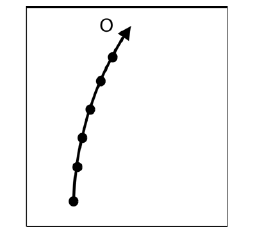
\includegraphics[scale=1]{immagini/minkowski/linea_universo}
   \caption{Linea di universo di un osservatore. I punti sono i ``battiti'' del suo orologio.}
\end{figure}

Per indagare l'universo fuori dalla sua piattaforma, l'osservatore non usa
più i regoli rigidi di Newton, bensì i segnali luminosi, scelti per la loro caratteristica 
di essere i segnali che si propagano alla velocità (limite) della luce\footnote{Inoltre, come si vedrà più avanti
nel capitolo relativo alle conferme sperimentali della relatività speciale ed ai paradossi relativistici, 
il modello di corpo rigido va in crisi in ambito relativistico.}. 
Per individuare un evento $E$ fuori dalla linea di universo dell'orologio, l'osservatore 
invia un segnale luminoso al tempo $T_1$, misurato dal suo orologio, in
modo tale che il segnale arrivi nel punto di accadimento dell'evento $E$ esat-
tamente quando $E$ accade, e poi misura il tempo di arrivo $T_2$ dell'eco riflessa.
La situazione è chiarita anche dalla figura \ref{radar1}, questa procedura è anche detta
\textbf{metodo dei segnali radar} o semplicemente ``metodo radar''.

\begin{figure}[htbp]
   \centering
   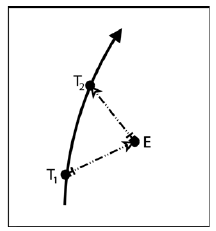
\includegraphics[scale=1]{immagini/minkowski/radar1}
   \caption{\label{radar1} Individuazione di un evento. Per convenzione indicheremo i segnali luminosi con queste particolari frecce trattopuntate.}
\end{figure}

I regoli di Newton sono stati sostituiti da ``regoli di luce'' e tutte le misure
sono ricondotte a misure di tempo eseguite con un unico orologio posto nella
piattaforma dell'osservatore locale.

\subsection{Misure di spazio, misure di tempo}
Il fatto di ricondurre tutte le misure spaziali a misure di tempo (cosa che
accade con questo ``metodo radar''), è un'ampliamento di prospettive e una
semplificazione concettuale. Possiamo portare come esempio quanto scrive
H. Bondi:
\begin{quote}
``Immaginiamo una civiltà in cui il metro sia sconosciuto e ogni distanza espressa in secondi-luce o 
millimicrosecondi-luce o in qualsiasi altra unità opportuna; i membri di questa società considererebbero
piuttosto sciocco chi chiedesse il valore della velocità della luce, essi
non la considererebbero una quantità da esprimere in metri al secondo
o chilometri al secondo, ma semplicemente come una unità, l'unità
naturale di velocità. La velocità di un oggetto verrebbe misurata paragonandola 
a quella della luce: tutte le velocità ordinarie sarebbero
espresse in termini di questo campione. [...] In altre parole accettando 
come campione di velocità [...] la velocità della luce, questa
civiltà avrebbe eliminato la necessità di costruire oltre a un campione
di tempo anche uno di lunghezza, e di usare uno scomodo numero per
esprimere la velocità della luce. In questa civiltà esisterebbe solo un
campione di tempo, i suoi componenti ci considererebbero delle persone 
che lavorano con lunghezze e tempi nel modo più complicato e
assurdo.''

(Hermann Bondi, La relatività e il senso comune, Zanichelli, pp. 36-37)
\end{quote}

Si consideri infatti:
\begin{quote}
``[...] una civiltà in cui la direzione nord-sud viene considerata sacra
ed è sempre misurata in miglia, mentre quella est-ovest viene considerata 
volgare e profana ed è sempre misurata in yarde. Se la gente
venisse abituata a vedere le cose sotto questo aspetto fin dalla prima
età, occorrerebbe una mente audace per suggerire l'esistenza di un
qualche legame tra le distanze nella direzione nord-sud e quelle nella
direzione est-ovest.''

(ibidem, p. 37)
\end{quote}

La stessa cosa accade dunque per noi: abbiamo sempre concepito spazio
e tempo come entità separate, cosicchè ci è costata fatica vederle come varie
declinazioni di un unico spaziotempo. In un'ottica unitaria di questo tipo
non c'è alcuna ragione di considerare anche un campione di lunghezza (come
ad esempio un regolo graduato): ci basta usare un campione di tempo, che
legheremo poi mediante $c$ alle quantità spaziali.

\section{Osservatori localmente inerziali}
Fin qui non vi è alcun modo di privilegiare un osservatore rispetto ad un
altro. Però possiamo constatare fisicamente che esiste una classe privilegiata
di osservatori locali, che chiameremo osservatori localmente inerziali.
Consideriamo, ad esempio, una navicella spaziale che navighi a motori spenti
in un'orbita interplanetaria. L'esperienza mostra che all'interno della navicella 
tutto avviene come previsto dalla teoria newtoniana degli osservatori
inerziali: due particelle lasciate libere o stanno ferme o si muovono di moto
rettilineo uniforme, un giroscopio messo in rotazione ha l'asse in direzione
invariabile, e così via. Ammettiamo perciò, come primo assioma, l'esistenza
di osservatori localmente inerziali (ove l'avverbio ``localmente'' si riferisce al
fatto che le osservazioni sono sempre locali, in un intorno dell'osservatore),
gli osservatori che cioè, sulla loro piattaforma, vedono le particelle libere soddisfare 
al principio di inerzia, i giroscopi in rotazione avere l'asse in direzione fissa, e così via.
Una questione interessante è comprendere l'origine degli osservatori inerziali. 
La risposta accettata oggi è che gli osservatori inerziali sono determinati 
dalla distribuzione di massa nell'universo (principio o punto di vista di
Mach\footnote{Ernst Mach (1838-1916), filosofo e fisico austriaco di grande influenza su Einstein e su
tutto il pensiero moderno.}). Una conferma di questo punto di vista viene dall'osservazione sperimentale 
la quale mostra che, rispetto a tali osservatori, il complesso delle
stelle che popolano l'universo appare fisso (e non ruotante): questo ci dice che
c'è una relazione misteriosa tra questi osservatori e la materia nell'universo.
Quindi l'origine degli osservatori localmente inerziali, detti anche osservatori
in caduta libera, starebbe in una proprietà globale dell'universo e dello spaziotempo 
che lo rappresenta. 

Gli osservatori localmente inerziali si riconoscono sperimentalmente facendo semplici 
esperienze meccaniche con particelle libere, che devono essere o ferme o muoversi di moto uniforme, con oscillatori, 
che non devono allungarsi, e con giroscopi, il cui asse non deve cambiare direzione.

Introdotti gli osservatori localmente inerziali, si studia poi il loro assemblamento 
(ossia come essi sono collegati). Consideriamo due osservatori inerziali
$O$ e $O'$ . Mediante il metodo dei segnali radar ognuno dei due può decidere se
l'altro è in quiete o in moto rispetto a lui. La condizione di quiete è espressa
dall'invarianza dell'intervallo di tempo T tra emissione e ricezione del segnale
radar, scambiato tra i due osservatori (come mostra la figura \ref{osservatori_radar} qui sotto).

\begin{figure}[htbp]\label{osservatori_radar}
   \centering
   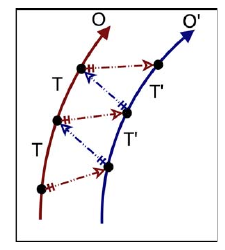
\includegraphics[scale=1]{immagini/minkowski/osservatori_radar}
   \caption{Scambio reciproco di segnali luminosi tra osservatori.}
\end{figure}

La proprietà vale tanto per il primo quanto per il secondo osservatore. Si
constata inoltre che se gli osservatori sono “suffientemente” vicini (situazione 
corrispondente a periodi $T$ e $T'$ ``sufficientemente'' piccoli) è possibile
calibrare gli orologi dei due osservatori in modo tale che $T$ = $T'$. Questo
processo di calibrazione prende il nome di sincronizzazione degli orologi
inerziali in quiete relativa.
Riepilogando: l'esperienza mostra che esistono osservatori localmente
inerziali in quiete relativa che possono essere sincronizzati tra loro. Rimane
aperto il problema dell'estensione di questo processo. Il processo di sincronizzazione 
di osservatori inerziali in grande è in generale impossibile. Tale
processo funziona solo per osservatori ``sufficientemente'' vicini: quando si
superano certe distanze e certi intervalli di tempo, cominciano a comparire 
delle discrepanze e si manifesta l'impossibilità di sincronizzare in grande
osservatori localmente inerziali nel modo prima descritto.

\section{Lo spaziotempo di Minkowski}
Si chiama spaziotempo di Minkowski uno spaziotempo ideale in cui si ammette 
che il processo di sincronizzazione prima descritto valga in grande. Lo
spaziotempo di Minkowski è quindi il modello di spaziotempo dove esistono
osservatori globalmente inerziali, costituiti da una rete di osservatori localmente inerziali 
in quiete relativa, sempre nel senso dello scambio di segnali
luminosi, e sincronizzati tra loro.

Lo spaziotempo di Minkowski è quindi un'approssimazione dello spazio-tempo fisico 
che può essere paragonata all'approssimazione che lo spazio tan-
gente fornisce di una superficie curva in un suo punto.

Nello spazio tangente possiamo parlare di rette e di rette parallele, mentre
sulla superficie possiamo solo parlare di geodetiche.Infatti le rette rimangono parallele 
in ogni punto dello spazio tangente, mentre le corrispondenti
geodetiche divergono sulla superficie a causa della curvatura della superficie.

Le rette e le geodetiche devono essere confrontate con le linee di universo degli
osservatori localmente inerziali nello spaziotempo. Rette parallele corrispon\-dono
ad osservatori inerziali in quiete relativa. Nello spaziotempo di Minkowski 
(corrispondente allo spazio tangente) queste linee di universo rimangono
sempre parallele, nello spaziotempo fisico invece no, a significare che dopo
un po' il processo di sincronizzazione diventa impossibile. L'impossibilità di
definire mediante il processo di sincronizzazione un osservatore globalmente
inerziale è quindi una misura della ``curvatura'' dello spaziotempo.

Nel modello di Minkowski, invece, si assume che esistano osservatori globalmente inerziali; 
ciò corrisponde a sviluppare una teoria dello spaziotempo
piatto. Questa teoria è la Relatività Ristretta. Essa è una buona approssimazione 
del mondo fisico in una scala di misure sulla quale si possono
trascurare gli effetti delle forze gravitazionali. La fisica nello spazio di Minkowski 
è, in sostanza, una fisica in assenza di gravità: in questa situazione è
possibile il processo di sincronizzazione prima descritto.
Su scale più grandi, dove non è possibile trascurare l'effetto delle forze
gravitazionali prodotte dalle grandi masse distribuite nell'universo, le forze
gravitazionali si manifestano come cause distorcenti il processo di sincronizzazione 
(influenti sul moto dei segnali luminosi), cosicchè l'approssimazione
dello spaziotempo di Minkowski non risulta più valida e bisogna passare all Relatività Generale. 
In sostanza, la Relatività Generale è la geometria dello spazio tempo quando si 
tiene conto dell'impossibilità della sincronizzazione in grande di osservatori
localmente inerziali.

Riassumendo:
\begin{itemize}
 \item il concetto di osservatore ha validità locale ed esistono degli osservatori
privilegiati detti localmente inerziali;
 \item in una prima approssimazione, è possibile parlare di osservatori localmente 
inerziali in quiete relativa e sincronizzare i rispettivi orologi in 
modo che misurino lo stesso periodo nei segnali scambiati;
 \item questo processo di sincronizzazione è solamente locale. Una buona
approssimazione dello spaziotempo reale è fornita dal modello ideale
in cui si ammette che la nozione di quiete relativa e il processo di
sincronizzazione abbiano validità globale. Questa proprietà definisce lo
spaziotempo di Minkowski.

\end{itemize}

\subsection{Il cono luce}

Immaginiamo di considerare nello spaziotempo di Newton due osservatori
inerziali in moto relativo l'uno rispetto all'altro, muniti dello stesso dispo-
sitivo per lanciare palline (pensate come punti materiali). Supponiamo che
a un certo istante i due osservatori si trovino nello stesso luogo (chiamiamo
questo evento $O$), e che lancino insieme le due palline. Le figure \ref{palline_raggi}
mostrano che cosa accade e che cosa accadrebbe se invece di lanciare pal\-line 
nello spazio newtoniano lanciassero segnali luminosi secondo la visione
di Einstein.

\begin{figure}[htbp]\label{palline_raggi}
   \centering
   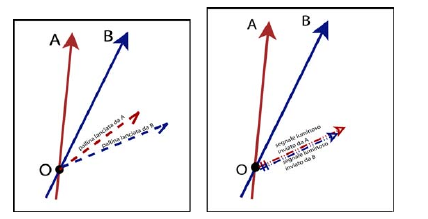
\includegraphics[scale=1]{immagini/minkowski/palline_raggi}
   \caption{A sinistra: palline lanciate da osservatori inerziali in moto rela-
tivo in un universo newtoniano. A destra: segnali luminosi inviati dagli stessi
osservatori inerziali in moto relativo in un universo einsteiniano.}
\end{figure}

Nel caso newtoniano, la velocità degli oggetti lanciati dipende dalla velocità della sorgente, 
e quindi le linee di universo delle palline lanciate da $A$ e $B$ nell'evento $O$, in generale, differiscono. Dunque non vi 
è alcuna linea di universo privilegiata rispetto alle altre.

Viceversa, nel caso di Einstein, il postulato riguardo all'invarianza di $c$
richiede che la velocità della luce non dipenda dalla velocità della sorgente.

Quindi due raggi luminosi, inviati in una data direzione da due sorgenti
che viaggiano con velocità diverse, viaggeranno comunque con la medesima
velocità. Il che equivale a dire che per ogni direzione spaziale vi è un'unica e
ben determinata linea di universo del segnale luminoso. 
L'insieme di queste linee di universo forma il ``cono luce'' associato all'evento considerato (v. figura
\ref{coni_luce}). 

\begin{figure}[htbp]
   \centering
   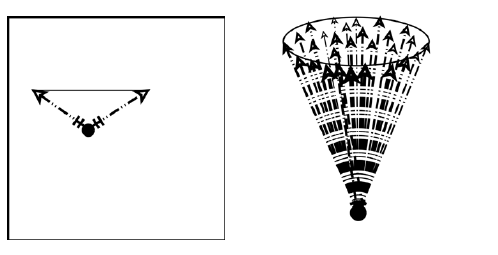
\includegraphics[scale=1]{immagini/minkowski/coni_luce}
   \caption{\label{coni_luce}Coni luce in universi (rispettivamente) bidimensionale e tridimen-
sionale. In un universo bidimensionale i possibili raggi inviati sono solamente due.}
\end{figure}

Nel caso di un universo bidimensionale, essendoci solo due direzioni
possibili per il raggio luminoso, il cono luce degenera a una sorta di triangolo.

\subsection{$c$ come velocità limite}

Lo spazio di Minkowski è utile per dare un significato geometrico alla relatività speciale.
Per comodità grafiche consideriamo solo una coordinata spaziale e una temporale. Sull'asse delle ascisse rappresentiamo $x$ 
e sull'asse delle ordinate, che chiamiamo $w$ il tempo moltiplicato per $c$, che lo rende uno spazio.
La bisettrice dei quadranti ha equazione:
\begin{equation}
 x = w = ct
\end{equation}
ed è la linea di universo della luce, essa rappresenta il cammino di un raggio luminoso.

Invece la linea di universo di un qualsiasi corpo dotato di massa che si muove con velocità $v$ dovrà avere
coefficiente angolare dato da:
\begin{equation}
\frac{\ud w}{\ud x}=\frac{\ud(ct)}{\ud x}=c\frac{1}{\frac{\ud x}{\ud t}}=\frac{c}{v}>1 
\end{equation}

Quindi la traiettoria di ogni punto massivo nel piano di Minkowski deve avere tangente in ogni 
punto maggiore di uno, altrimenti andrebbe più veloce della luce.

\subsection{Osservatori nello spaziotempo di Minkowski}

Creiamo un nuovo sistema di riferimento inerziale.
Partiamo dalle trasformazioni di Lorentz:
\begin{equation}
\left\{\begin{array}{l}
x'=\frac{x-ut}{\sqrt{1-\beta^2}}\\
t'=\frac{t-\frac{\beta}{c}x}{\sqrt{1-\beta^2}}\\
\end{array}\right. 
\end{equation}

Se moltiplichiamo e dividiamo per $c$ ogni qual volta che abbiamo una velocità, ricordando che
$w = ct$ e $\beta = \frac{u}{c}$, abbiamo che:
\begin{equation}\label{x_w_to_xp_wp}
\left\{\begin{array}{l}
x'=\frac{x-\beta w}{\sqrt{1-\beta^2}}\\
w'=\frac{w-\beta x}{\sqrt{1-\beta^2}}\\
\end{array}\right. 
\end{equation}

Se vogliamo disegnare il nuovo sistema di riferimento $(x', w')$ 
dobbiamo ricavarne le equazioni rispetto al sistema di riferimento $(x, w)$
quindi:
\begin{equation}
\left\{\begin{array}{l}
\text{asse} \; x': w'=0 \\
w'=\frac{w-\beta x}{\sqrt{1-\beta^2}}\\
\end{array}\right. 
\qquad
\left\{\begin{array}{l}
x'=\frac{x-\beta w}{\sqrt{1-\beta^2}}\\
\text{asse} \; w': x'=0
\end{array}\right.  
\end{equation}
Da cui si ricavano le equazioni degli assi $x'$, $w'$:
\begin{equation}
 \left\{\begin{aligned}
  &\text{asse} \; x': &w &=\beta x \\
  &\text{asse} \; w': &w &= \frac{1}{\beta } x  \\
 \end{aligned}\right.  
\end{equation}

Più $\beta$ tende a $1$ e più i due assi del nuovo sistema di riferimento tendono alla bisettrice del primo--terzo quadrante.

I sistemi che abbiamo costruito sono rappresentati nella figura \ref{Mink2}.
\begin{figure}
   \centering
   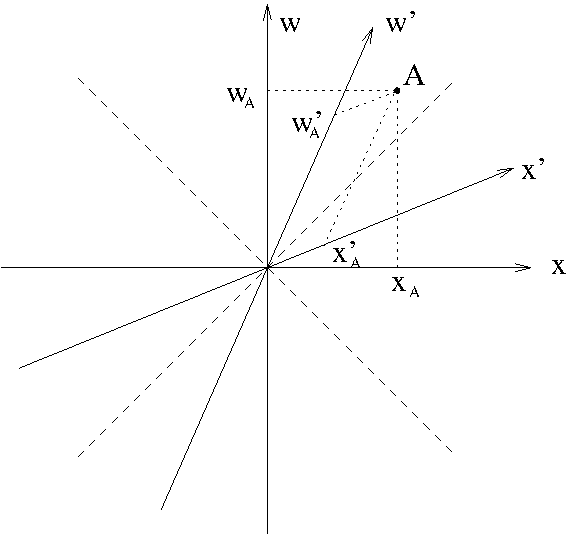
\includegraphics[scale=1]{immagini/minkowski/Mink2}
   \caption{\label{Mink2} ``Costruzione'' di un osservatore nello spaziotempo di Minkowski.}
\end{figure}


\subsubsection{Curve di calibrazione\index{curve! di calibrazione}}

Come rappresentato in figura \ref{Mink2} posso rappresentare un osservatore con un sistema di riferimento cartesiano.
L'osservatore che riteniamo fermo è rappresentato dagli assi $x \hat O w$, quello in moto dagli assi $x' \hat O' w$. Indichiamo 
le coordinate rispetto al sistema $x \hat O w$ con $(x,w)$ e quelle rispetto al sistema $x' \hat O' w$ con $(x',w')$.

Per trasportare una misura da un sistema all'altro è necessario applicare le trasformazioni di Lorentz, per facilitare questo
processo si disegnano le ``curve di calibrazione''.  Esse sono date dalle seguenti equazioni:
\begin{equation}
\left\{\begin{array}{l}
x^2 - w^2 =  1\\
x^2 - w^2 = -1\end{array}\right. 
\end{equation}

\begin{figure}[htbp]
   \centering
   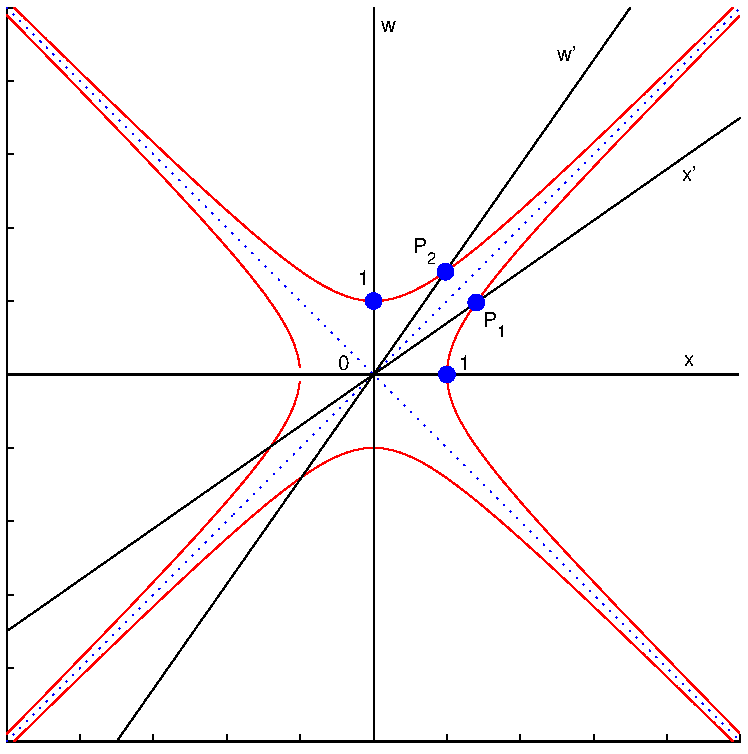
\includegraphics[scale=0.7]{immagini/minkowski/Minkowski_calibrazione}
   \caption{\label{Minkowski_calibrazione}Curve di calibrazione nello spaziotempo di Minkowski.}
\end{figure}


Queste curve, rappresentate nella figura \ref{Minkowski_calibrazione}, ci permettono di trasportare il segmento 
unitario nella direzione spaziale o temporale del sistema $x \hat O w$ a quello del sistema  $x' \hat O' w$.

Infatti il punto $P: (1, 0)$ ovvero l'unità di lunghezza nel sistema $x \hat O w$ viene trasportata nel punto $P'$
le cui coordinate sono date da:
\begin{equation}
\left\{\begin{array}{l}
x^2-w^2=1\\
\text{asse} \; x': w'=0 \rightarrow w =\beta x \\
\end{array}\right. 
\end{equation}

da cui si ricavano le coordinate di $P'$ rispetto al sistema $x \hat O w$, ovvero\footnote{Ricordiamo che $0 \leq \beta < 1 $, 
quindi le relazioni sono ben definite}:
\begin{equation}
P' \left\{\begin{aligned} 
x &= \frac{1}{\sqrt{1-\beta^2}}\\
w &= \frac{\beta}{\sqrt{1-\beta^2}}
\end{aligned}\right. 
\end{equation}
Il punto $P'$ corrisponde a $(1', 0')$, ossia
all'unità di lunghezza nel sistema $x' \hat O' w$, infatti usando \ref{x_w_to_xp_wp}:
\begin{equation}
 \left\{
 \begin{aligned}
 x' &= \dfrac{\dfrac{1}{\sqrt{1-\beta^2}}-\beta w}{\sqrt{1-\beta^2}} = \dfrac{\dfrac{1}{\sqrt{1-\beta^2}}-\dfrac{\beta^2}{\sqrt{1-\beta^2}}}{\sqrt{1-\beta^2}} = 1 \\
 w' &= \dfrac{\beta}{\sqrt{1-\beta^2}} - \beta \dfrac{1}{\sqrt{1-\beta^2}} = 0
 \end{aligned}
 \right. 
\end{equation}

Da questi diagrammi è possibile ottenere in modo diverso gli effetti di dilatazione dei tempi e di contrazione delle lunghezze.

\subsubsection{Le trasformazioni di Lorentz come rotazioni iperboliche\index{le trasformazioni di Lorentz! come rotazioni iperboliche}}


\subsection{La struttura di causalità dello spaziotempo}
La velocità della luce è invariante, ma abbiamo anche postulato che sia una
velocità limite, ovvero che non esistano sistemi o segnali fisici che possano
oltrepassare tale velocità. Questa proprietà ci è utile per stabilire la relazione
tra osservatori inerziali e coni luce.

La questione che ci poniamo è: come sono disposte le linee di universo
degli osservatori inerziali rispetto ai coni luce? La risposta è che le linee
di universo di tali osservatori devono necessariamente cadere all'interno del
cono, poichè essendo $c$ velocità limite, un segnale che viaggiasse al di fuori
dal cono avrebbe pendenza minore, e dunque una velocità maggiore di $c$.

\begin{figure}[htbp]
   \centering
   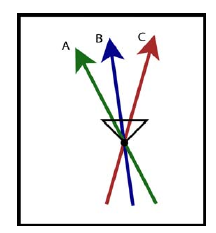
\includegraphics[scale=0.7]{immagini/minkowski/osservatori_coni_luce2}
   \caption{\label{osservatori_coni_luce2} Possibili linee di universo per osservatori massivi.}
\end{figure}

\begin{figure}[htbp]
   \centering
   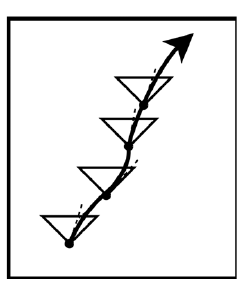
\includegraphics[scale=0.7]{immagini/minkowski/osservatori_coni_luce3}
   \caption{Da ogni punto dello spazio tempo possiamo fare partire un cono luce.}
\end{figure}


Il carattere di velocità limite di $c$ implica quindi che le linee di universo degli 
ossevatori inerziali siano contenute nel cono luce. Queste linee di universo
sono dette linee del genere tempo. Da questa osservazione segue subito la divisione (relativamente a un
evento prefissato $O$) dello spaziotempo $M$ in tre regioni distinte (v. figura
\ref{struttura_causale}):

\begin{figure}[htbp]
   \centering
   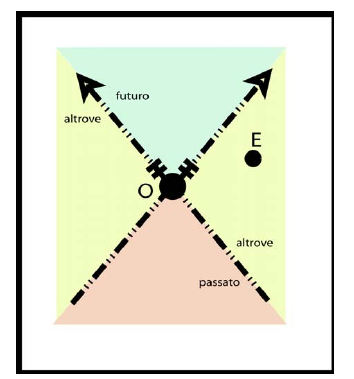
\includegraphics[scale=0.7]{immagini/minkowski/struttura_causale}
   \caption{\label{struttura_causale} La ``struttura causale'' dello spaziotempo.}
\end{figure}

\begin{itemize}
 \item futuro: è la falda del cono che contiene le linee del genere tempo, nel
senso dell'orientamento delle linee di universo degli osservatori;
 \item passato: l'altra falda del cono;
 \item altrove: tutta la parte rimanente dello spaziotempo
\end{itemize}

Questa distinzione ha un significato fisico profondo: distingue gli eventi
che possono essere influenzati da $O$ (futuro) dagli eventi che possono aver
influenzato $O$ (passato) e da quelli che non possono essere messi in relazione
causale con $O$ (altrove). Vedremo infatti che, se possiamo dare un ordinamento 
temporale per gli eventi del futuro e del passato (possiamo dire quindi
univocamente se $E$ avviene prima o dopo $O$, nel senso che tutti gli osservatori
concordano su ciò), a eventi situati nell'altrove non riusciremo ad attribuire
una consequenzialità temporale: ci saranno osservatori che li diranno simultanei a O, 
altri che li vedranno accadere prima di $O$, altri ancora che li
vedranno accadere dopo $O$.

L'assioma riguardo all'invarianza di $c$ si traduce geometricamente in modo molto
particolare, esso infatti è la prima struttura geometrica dello spaziotempo di Minkowski 
(indicato con $M$) , detta ``struttura di causalità'', poichè
essa regola il segno del divario temporale tra gli eventi, e quindi stabilisce
l'ordinamento temporale che è alla base del principio di causa-effetto. Se
vogliamo affermare, infatti, che un evento $A$ è causa di un evento $B$, deve
quantomeno sussistere il fatto che $A$ accada prima di $B$. Per confronto con
la cinematica newtoniana, vediamo che cosa implica l'assioma dell'invarianza
di $c$ nella geometria di $M$.

\subsection{Coordinate di un evento}
Stabilita la traduzione geometrica degli assiomi, cominciamo a vedere come
ogni osservatore inerziale individua, con le sue coordinate relative, ogni evento;
in linguaggio geometrico, costruiamo il sistema di coordinate globali su $M$
associato ad un dato osservatore inerziale. Non ci sono più regoli, e quindi il
meccanismo è interamente basato sui segnali luminosi.

Dato un osservatore $A$, innanzitutto introduciamo le coordinate radar
$(T_1 , T_2)$ dell'evento $E$, definite facendo riferimento ancora alla figura
\ref{osservatori_radar} come segue:
\begin{itemize}
 \item $T_1$: è il tempo di emissione (rispetto all'orologio dell'osservatore A) del
segnale luminoso emesso da $A$ che giunge in $E$;
 \item $T_2$: è il tempo di ricezione del segnale riflesso (sempre nel giudizio di $A$).

\end{itemize}

In linguaggio geometrico, le coordinate radar non sono nient'altro che le
intercette del cono luce di vertice $E$ con la linea di universo dell'osservatore
$A$.
Si passa poi alle coordinate spaziotemporali $(x, t)$ dell'evento mediante le
seguenti definizioni:
\begin{equation}
 \begin{aligned}{ll}
  ct &= \dfrac{1}{2} c(T_2 + T_1 ) \\
  x &= \dfrac{1}{2} c(T_2 - T_1 )
 \end{aligned}
\end{equation}

Sostanzialmente stiamo definendo il tempo dell'evento $E$ come media dei
due tempi (tempo di emissione e tempo di ricezione), e come spazio lo spazio
percorso dal raggio luminoso nella semisomma dei tempi, ossia nella metà
del periodo emissione-ricezione.

Occorre puntare l'attenzione sul fatto che tali definizioni sono le uniche
definizioni plausibili con le informazioni in nostro possesso (solo $T_1$ , $T_2$ e
$c$), ipotizzando tacitamente che lo spazio sia isotropo, ossia che la velocità
della luce non cambi tra andata e ritorno. Non abbiamo altra scelta che
prendere come tempo il tempo medio di riflessione: secondo il punto di vista
dell'osservatore $A$, la luce, per giungere ad $E$, deve impiegare lo stesso tempo
che impiega per tornare indietro.

\subsection{L'effetto Doppler longitudinale}
Veniamo ora al problema centrale della nostra analisi: quello del confronto tra diversi 
osservatori inerziali in moto relativo, passo indispensabile per la scoperta delle 
caratteristiche comuni ai vari osservatori e della geometria dello spaziotempo.

Il nucleo della questione è il confronto tra gli orologi dei due osservatori
in moto. Questo confronto è fatto misurando il periodo di emissione e il
periodo di ricezione (ognuno nel giudizio del corrispondente osservatore) in un
processo di scambio di segnali luminosi periodici - essendo i segnali luminosi
l'unico mezzo che gli osservatori hanno a disposizione per confrontarsi.

Sia $T_e$ il periodo di emissione nel giudizio di $A$, e sia $T_r$ il periodo di
ricezione valutato da $B$. Se $B$ si allontana da $A$ con velocità 
relativa\footnote{Si presti attenzione a questo particolare: se avessimo a che fare con l'effetto Doppler acustico
(cioè il fenomeno per cui un suono cambia frequenza all'avvicinarsi/allontanarsi di sorgente o osservatore) 
non potremmo considerare solo la velocità relativa tra sorgente e osservatore.
Avendo, infatti, l'onda sonora bisogno di un mezzo (l'aria) per propagarsi, è necessario
considerare le velocità rispetto all'aria sia della sorgente, sia dell'osservatore. Nella nostra
analisi radar, invece, tutto questo non è necessario: l'onda elettromagnetica non ha bisogno 
di alcun mezzo per propagarsi. Quindi l'effetto Doppler relativistico è molto più
semplice da trattare rispetto a quello ``classico'' (acustico)} $v$,
deve necessariamente essere che $T_r > T_e$ , poichè il secondo segnale ha dovuto
percorrere una distanza maggiore per raggiungere $B$. In generale, poniamo
\begin{equation}
T_r = k(v) \cdot Te  
\end{equation}
con $k(v) > 0$ funzione della velocità relativa $v$ tra i due
osservatori. Avremo che $k > 1$ se i due osservatori si allontanano, $k = 1$ se
i due osservatori sono in quiete relativa, $0 < k < 1$ se i due osservatori si
avvicinano. Il fattore $k$, termine centrale nel nostro studio (da cui, appunto,
il nome di $k$-calcolo), viene detto ``fattore 
Doppler\footnote{Christian Johann Doppler (1803-1853), fisico austriaco.}
 longitudinale'', l'aggettivo ``longitudinale'' sta ad indicare che i segnali luminosi sono emessi
nella direzione del moto relativo dei due osservatori.

Disponiamo solamente di due informazioni:
\begin{enumerate}
 \item $B$ si muove di moto relativo con velocità $v$ rispetto ad $A$;
 \item il Principio di Relatività;
\end{enumerate}
Queste informazioni sono sufficienti per risolvere il problema. 
Supponiamo infatti di avere due osservatori in moto relativo $B$ ed 
$A$, come descritto dalla figura \ref{doppler}. Secondo l'osservatore
$A$, $B$ si muove secondo la legge:
\begin{equation}\label{moto_relativo}
x=vt 
\end{equation}
con $(x, t)$ coordinate di $B$ nel giudizio di $A$.

\begin{figure}[htbp]
   \centering
   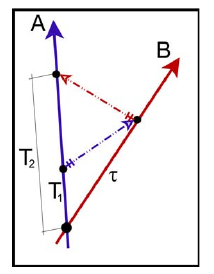
\includegraphics[scale=1]{immagini/minkowski/doppler}
   \caption{\label{doppler} Doppio scambio Doppler. Gli istanti temporali 
sono interpretati come periodi di tempo del doppio scambio Doppler
tra $A$ e $B$: $T_1$ è il periodo di emissione da parte di $A$ di un segnale periodico
ricevuto da $B$ con un periodo di ricezione $\tau$; $T_2$ è il periodo di ricezione da
parte di $A$ di un segnale periodico emesso da $B$ con un periodo $\tau$.}
\end{figure}

Il nodo centrale è interpretare la figura \ref{doppler} dal punto di vista dell'effetto
Doppler, convenendo che $A$ e $B$ si scambino un primo segnale (una sorta di
``azzeramento'' degli orologi) in $O$. In questo modo convertiamo le coordinate
radar in periodi.

Ciò che succede è che $A$ e $B$ sincronizzano gli orologi quando si incontrano;
dopo un tempo $T_1$ (nel giudizio di $A$), $A$ lancia un segnale luminoso che arriva
al tempo $\tau$ (nel giudizio di $B$) all'osservatore $B$, il quale lo rispedisce subito
indietro. Il segnale ritorna al tempo $T_2$, nel giudizio di $A$, all'osservatore $A$.
Il diagramma \ref{doppler} del moto relativo serve a localizzare $B$ nel giudizio di
$A$. Infatti ($T_1$ , $T_2$) sono esattamente le coordinate radar di $B$, in particolare
sono le coordinate dell'evento $E$ ``ricezione del segnale da parte di $B$'', rispetto ad $A$. 
Quindi le equazioni:
\begin{equation}
 \begin{array}{ll}
  ct &= \frac{1}{2} c(T_2 + T_1) \\
  x &= \frac{1}{2} c(T_2 - T_1)
 \end{array}
\end{equation}
forniscono la posizione e il tempo di $B$ nel giudizio di $A$. 
Unendo questo risultato all'informazione \ref{moto_relativo}, possiamo scrivere che
\begin{equation}\label{doppler1}
 \dfrac{v}{c} = \dfrac{x}{ct} =\dfrac{T_2 - T_1}{T_2 + T_1} 
\end{equation}

Ora colleghiamo le coordinate radar con il fattore Doppler, osservando
che $\tau$, nel grafico dello scambio Doppler, è esattamente il periodo di ricezione
da parte di $B$ di un treno d'onde emesso da $A$ con periodo $T_1$ abbiamo:
\begin{equation}\label{doppler2}
\tau = k_{AB} (v) \cdot T_1
\end{equation}
con $k_{AB} (v)$ fattore Doppler longitudinale quando $A$ emette e $B$ riceve. Allo
stesso modo, posso interpretare $T_2$ come periodo di ricezione da parte di $A$ di
un treno d'onde emesso da $B$ con periodo $\tau$, ne deduciamo che:
\begin{equation}\label{doppler3}
T_2 = k_{BA} (v) \cdot \tau
\end{equation}
con $k_{BA} (v)$ fattore Doppler longitudinale quando $B$ emette e $A$ riceve.
Ma il Principio di Relatività impone che ci sia completa simmetria tra
$A$ e $B$, ovvero che\footnote{Il simbolo $:=$ significa ``per definizione''}:
\begin{equation}
k_{BA} (v) = k_{AB} (v) := k(v).
\end{equation}
Se non fosse così infatti, avremmo modo di scegliere un osservatore privilegiato, ad esempio, 
l'osservatore che ha il minor $k$ quando emette i segnali luminosi).
Ne deduciamo che devono valere le seguenti tre equazioni \ref{doppler1}, \ref{doppler2},
\ref{doppler3} si ricava quindi che:
\[
 \dfrac{v}{c} = \dfrac{k - k^{-1}}{k + k^{-1}} = \dfrac{k^2 -1}{k^2 +1}
\]
ovvero: $vk^2 + v = ck^2 - c$, da cui
\begin{equation}
k = \sqrt{\dfrac{c+v}{c-v}} 
\end{equation}
Dunque, se $B$ si allontana da A, abbiamo che $v > 0$, ovvero $k > 1$. Se $A$
e $B$ sono in quiete relativa, abbiamo che $v = 0$, ovvero $k = 1$. Se infine $B$ si
avvicina ad $A$, abbiamo che $v < 0, k < 1$.

